\documentclass[crop=false, class=book]{standalone}


\usepackage{graphicx}
\usepackage[italian]{varioref}
\usepackage{copyrightbox}


\begin{document}
	\chapter{Instant Placement}
	L'API di posizionamento istantaneo consente di posizionare gli oggetti nell’ambiente prima ancora che venga spostato il dispositivo e che vengano individuati i piani \cite{google2022instant}. \\
	\noindent
	Dopo che l’utente ha posizionato l’oggetto, la sua posizione viene perfezionata in tempo reale mentre l’utente si muove nell’ambiente.
	\\
	\noindent
	Successivamente, quando ARCore è in grado di identificare con precisione l’ubicazione dell’oggetto nello spazio, viene cambiata la sua posizione e dimensione per rispettare la scala dell’ambiente.
	\begin{figure}
		\centering
		\copyrightbox[b]{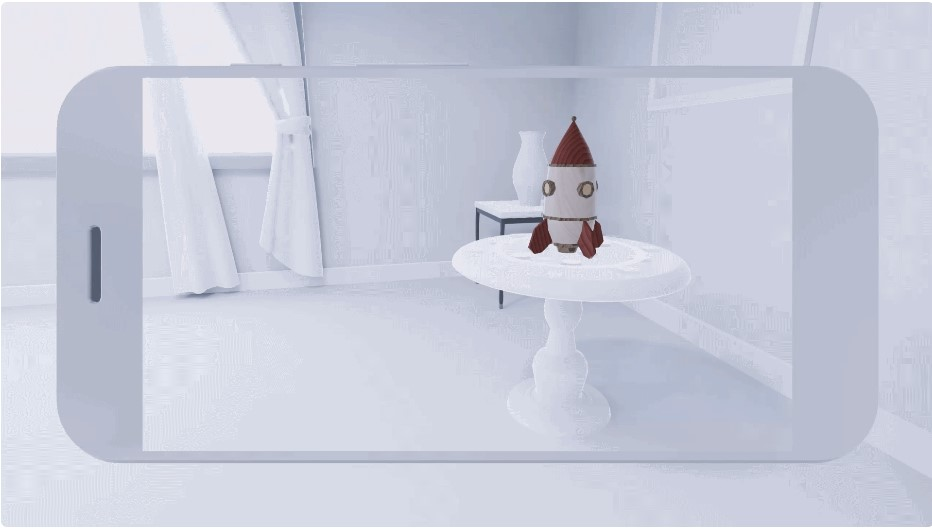
\includegraphics[width=0.6\textwidth]{./resources/images/InstantPlacement/InstantPlacementImg.jpg} }%
		{Fonte: \url{https://developers.google.com}}
		\caption{Instant Placement}
		\label{fig:instant}
	\end{figure}
	\\
	\noindent
	Per abilitare l’Instant Placement bisogna creare una sessione configurata per supportare tale funzionalità, come descritto dal listing~\vref{lst:ip_session} tratto dalla documentazione ufficiale \cite{google2022instant2}.
		
	\begin{center}
		\begin{minipage}{0.95\textwidth}
			\begin{lstlisting}[caption={Creazione della sessione ARCore con Instant Placement abilitato.}, label={lst:ip_session}, language=Kotlin]
			fun createSession() {
				
			val session = Session(applicationContext);
			
			val config = Config(session)
			
			config.instantPlacementMode = Config.InstantPlacementMode.LOCAL_Y_UP
			
			session.configure(config)
		}
		\end{lstlisting}
		\end{minipage}
	\end{center}

\end{document}